
\chapter{Basics of finite elements}

Many differential equations of interest cannot be solved exactly; however, they may be solved approximately if given some simplifying assumptions.  For example, perturbation methods approximate an \emph{inner} and \emph{outer} solution to a problem with different characteristic length or time scales, Taylor-series methods determine a locally convergent approximation, Fourier-series methods determine a globally-convergent approximation, and finite-difference methods provide an approximation over a uniformly discretized domain.  The finite element method is a technique which non-uniformly discretizes the domain of a variational or weighted-residual problem into \emph{finite elements}, which may then be assembled into a single matrix equation and solved for an approximate solution.

%===============================================================================

\section{Motivation: weighted integral approximate solutions} \label{ssn_intro_motivation}

Following the explanation in \citet{reddy_1993}, the approximation of a differential equation with unknown variable $u$ which we seek is given by the linear expansion
\begin{align}
  \label{intro_motivation_approximation}
  u(x) \approx \sum_{i=0}^N u_i \psi_i,
\end{align}
where $u_i$ are coefficients to the solution, $N$ is the number of parameters in the approximation, and $\psi$ is a set of linearly independent functions which satisfy the boundary conditions of the equation.  For example, consider the second-order differential equation
\begin{align}
  \label{intro_motivation_ode}
  - \totder{}{x} \left[ \totder{u}{x} \right] + u = 0, \hspace{5mm} 0 < x < 1,
\end{align}
\begin{align}
  \label{intro_motivation_bcs}
  u(0) = 1, \hspace{10mm} \left( \totder{u}{n} \right) \Bigg|_{x=1} = 0,
\end{align}
where $n$ is the outward-pointing normal to the domain.  In the 1D case here, $n(0) = -1$ and $n(1) = 1$.  The $N=2$ parameter approximation with
\begin{align*}
  \psi_0 = 1, \hspace{5mm} \psi_1 = x^2 - 2x, \hspace{2.5mm} \text{and} \hspace{2.5mm} \psi_2 = x^3 - 3x,
\end{align*}
in (\ref{intro_motivation_approximation}) gives the approximate solution
$$u(x) \approx U_N = u_0 + u_1 (x^2 - 2x) + u_2 (x^3 - 3x).$$
This approximation satisfies the \emph{Neumann} or \emph{natural} boundary condition
\index{Boundary conditions!Essential} \index{Boundary conditions!Natural}
at $x=1$, and in order to satisfy the \emph{Dirichlet} or \emph{essential} boundary condition at $x=0$, we make $u_0 = 1$, producing
\begin{align}
  \label{intro_motivation_expansion}
  u(x) \approx U_N = 1 + u_1 (x^2 - 2x) + u_2 (x^3 - 3x).
\end{align}
Substituting this approximation into differential equation (\ref{intro_motivation_ode}) results in
{\footnotesize
\begin{align*}
  - 2u_1(x - 1) - 3u_2(x^2 - 1) + 1 + u_1(x^2 - 2x) + u_2 (x^3 - 3x) &= 0 \\
  (2u_1 + 3u_2 + 1) - (2u_1 + 2u_1 + 3u_2)x - (3u_2 - u_1)x^2 + u_2x^3 &= 0,
\end{align*}}
implying that
\begin{align*}
  2u_1 + 3u_2 + 1 &= 0 \\
  4u_1 + 3u_2 &= 0 \\
  3u_2 - u_1 &= 0 \\
  u_2 &= 0.
\end{align*}
This system of equations has only the trivial solution $u=0$ and is hence inconsistent with differential equation (\ref{intro_motivation_ode}, \ref{intro_motivation_bcs}).  However, if the problem is evaluated as a \emph{weighted integral} it can be guaranteed that the number of parameters equal the number of linearly independent equations.  This weighted integral relation is
$$\int_0^1 w R \d{x} = 0,$$
where $R$ is the approximation residual of Equation (\ref{intro_motivation_ode}),
$$R = - \totder[2]{U_N}{x} + U_N,$$
and $w$ are a set of $N$ linearly independent \emph{weight functions}.  For this example we use
$$w_1 = x, \hspace{2.5mm} \text{and} \hspace{2.5mm} w_2 = x^2,$$
and two integral relations to evaluate,
{\scriptsize
\begin{align*}
  0 &= \int_0^1 w_1 R \d{x} = \int_0^1 x R \d{x} \\
    &= \left[ \frac{1}{2}(2u_1 + 3u_2 + 1)x^2 - \frac{1}{3}(4u_1 + 3u_2)x^3 - \frac{1}{4}(3u_2 - u_1)x^4 + \frac{1}{5}u_2x^5 \right]_0^1 \\
    &= \frac{1}{2}(2u_1 + 3u_2 + 1) - \frac{1}{3}(4u_1 + 3u_2)x^3 - \frac{1}{4}(3u_2 - u_1) + \frac{1}{5}u_2 \\
    &= \frac{1}{2} + \left( 1 - \frac{4}{3} + \frac{1}{4} \right) u_1 + \left( \frac{3}{2} - 1 - \frac{3}{4} + \frac{1}{5} \right) u_2 \\
    &= \frac{1}{2} - \frac{1}{12} u_1 - \frac{1}{20} u_2
\end{align*}}
and
{\scriptsize
\begin{align*}
  0 &= \int_0^1 w_2 R \d{x} = \int_0^1 x^2 R \d{x} \\
    &= \left[ \frac{1}{3}(2u_1 + 3u_2 + 1)x^3 - \frac{1}{4}(4u_1 + 3u_2)x^4 - \frac{1}{5}(3u_2 - u_1)x^5 + \frac{1}{6}u_2x^6 \right]_0^1 \\
    &= \frac{1}{3}(2u_1 + 3u_2 + 1) - \frac{1}{4}(4u_1 + 3u_2) - \frac{1}{5}(3u_2 - u_1) + \frac{1}{6}u_2 \\
    &= \frac{1}{3} + \left( \frac{2}{3} - 1 + \frac{1}{5} \right) u_1 + \left( 1 - \frac{3}{4} - \frac{3}{5} + \frac{1}{6} \right) u_2 \\
    &= \frac{1}{3} - \frac{2}{15} u_1 - \frac{11}{60} u_2,
\end{align*}}
giving a system of equations for the coefficients $u_1$ and $u_2$,
\begin{align*}
  \begin{bmatrix}
    - \frac{1}{12} & - \frac{1}{20} \\
    - \frac{2}{15} & - \frac{11}{60} \\
  \end{bmatrix} \cdot
  \begin{bmatrix}
    u_1 \\
    u_2
  \end{bmatrix} = 
  \begin{bmatrix}
    -\frac{1}{2} \\
    -\frac{1}{3}
  \end{bmatrix}.
\end{align*}
Solving this system produces $u_1 = \frac{270}{31}$ and $u_2 = \frac{-140}{31}$, and thus approximation (\ref{intro_motivation_expansion}) is given by
\begin{align}
  \label{intro_motivation_approximation_final}
  u_N(x) = 1 + \frac{270}{31} (x^2 - 2x) - \frac{140}{31} (x^3 - 3x).
\end{align}

\subsection{Exact solution}

Differential equation (\ref{intro_motivation_ode}) is easily solved exactly:
$$\totder[2]{u}{x} - u = 0 \hspace{2.5mm} \implies \hspace{2.5mm} u = c_1 \cosh(x) + c_2 \sinh(x)$$ 
$$u(0) = c_1 = 1, \hspace{5mm} u'(1) = \sinh(1) + c_2 \cosh(1) = 0$$
$$\implies c_2 = -\frac{\sinh(1)}{\cosh(1)} = -\tanh(1),$$
and 
\begin{align}
  \label{intro_motivation_exact}
  u(x) = \cosh(x) - \tanh(1)\sinh(x).
\end{align}

Weighted integral approximation (\ref{intro_motivation_approximation_final}) and exact solution (\ref{intro_motivation_exact}) are shown in Figure \ref{scratch_example_image}.

\pythonexternal[label=weight_int_plot, caption={Scipy source code used to generate Figure \ref{scratch_example_image}}]{scripts/fenics_intro/weight_int.py}

\begin{figure}
  \centering
    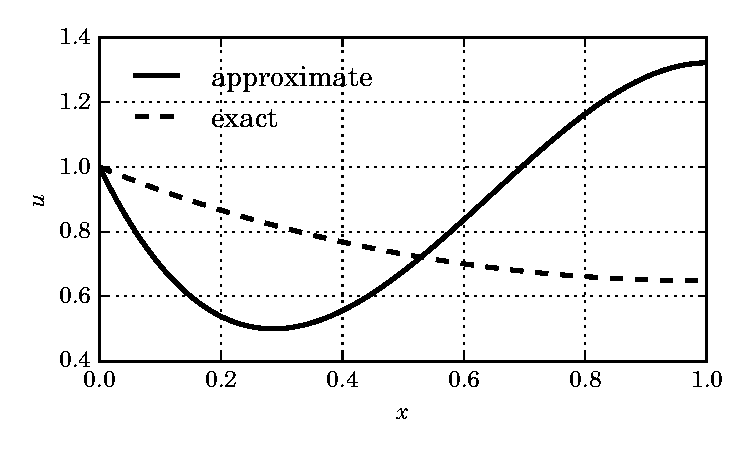
\includegraphics[width=\linewidth]{images/fenics_intro/weight_int.pdf}
  \caption[FEM intro scratch example]{Weighted integral approximation (solid) and exact solution (dashed).  Note that the approximation will be improved by increasing $N$.}
  \label{scratch_example_image}
\end{figure}

%===============================================================================

\section{The finite element method}

The finite element method combines variational calculus, Galerkin approximation methods, and numerical analysis to solve initial and boundary value differential equations \citep{reddy_1993}.  The steps involved in the finite element approximation of a typical problem are
\begin{enumerate}
  \item Discretization of the domain into finite elements.
  \item Derivation of element equations over each element in the mesh.
  \item Assembly of local element equations into a global system of equations.
  \item Imposition of boundary conditions.
  \item Numerical solution of assembled equations.
  \item Post processing of results.
\end{enumerate}

In the following sections, we examine each of these steps for the 1D-boundary-value problem \citep{davis_2013} over the domain $\Omega \in (0,\ell)$ with essential boundary $\Gamma_D$ at $x=0$ and natural boundary $\Gamma_N$ at $x=\ell$
\begin{align}
  \label{intro_ode}
  -\totder{}{x} \left[ k(x) \totder{u}{x} \right] &= f(x) && \text{ in } \Omega \\
  \label{intro_ode_nbc}
  \left( k(x) \totder{u}{n} \right) &= g_N && \text{ on } \Gamma_N \\
  \label{intro_ode_ebc}
  u &= g_D && \text{ on } \Gamma_D,
\end{align}
and develop a finite-element model from scratch.

\subsection{Variational form} \label{ssn_variational_form}

The variational problem \index{Variational form} corresponding to (\ref{intro_ode} -- \ref{intro_ode_ebc}) is formed by multiplying Equation (\ref{intro_ode}) by the weight function $w(x)$ and integrating over the $x$-coordinate domain $\Omega \in (0,\ell)$,
$$-\int_{\Omega} \totder{}{x} \left[ k(x) \totder{u}{x} \right] w(x) \d{\Omega} = \int_{\Omega} f(x) w(x) \d{\Omega},$$
with no restrictions on $w(x)$ made thus far.  Integrating the left-hand side by parts,
\begin{align*}
  \int_0^{\ell} k \totder{u}{x} \totder{w}{x} \d{x} - \left[ wk\totder{u}{n}\right]_0^{\ell} &= \int_0^{\ell} f w \d{x}.
\end{align*}
This formulation is called the \emph{weak form} \index{Weak form} of the differential equation due to the ``weakened'' conditions on the approximation of $u(x)$.

In the language of distributional solutions in mathematical analysis, the \index{Trial functions} \emph{trial} or \emph{solution function} $u$ is a member of the \emph{trial} or \emph{solution space} that satisfies the essential boundary condition $g_D$ on Dirichlet boundary $\Gamma_D$,
\begin{align}
  \label{trial_space}
  \mathcal{H}_E^1(\Omega) &= \left\{ u \in \mathcal{H}^1(\Omega)\ |\ u = g_D\ \text{on}\ \Gamma_D \right\},
\end{align}
while the \index{Test functions} \emph{test function} $w$ is member of the \emph{test space}
\begin{align}
  \label{test_space}
  \mathcal{H}_{E_0}^1(\Omega) &= \left\{ u \in \mathcal{H}^1(\Omega)\ |\ u = 0\ \text{on}\ \Gamma_D \right\}.
\end{align}
These spaces are both defined over the space of square-integrable functions whose first derivatives are also square integrable; the $\Omega \subset \R$ \index{Sobolev space} \emph{Sobolev space} \citep{elman_2005}
\begin{align}
  \label{sobolev_space}
  \mathcal{H}^1(\Omega) &= \left\{ u\ :\ \Omega \rightarrow \R\ \Bigg|\ u, \totder{u}{x} \in L^2(\Omega) \right\},\\
  \label{l2_space}
  L^2(\Omega) &= \left\{ u\ :\ \Omega \rightarrow \R\ \Bigg|\ \int_{\Omega} u^2 \d{\Omega} < \infty \right\},
\end{align}
where the space of functions in \index{L@$L^2$ space} $L^2(\Omega)$ is defined with the measure
\begin{align}
  \label{l2_norm}
  \Vert u \Vert_2 = \left( \int_{\Omega} u^2 \d{\Omega} \right)^{\nicefrac{1}{2}},
\end{align}
and the \index{Inner product} $L^2$ \emph{inner product} $(f,g) = \int_{\Omega} f g \d{\Omega}$.

The variational problem consists of finding $u \in \mathscr{H}_E^1(\Omega)$ such that
\begin{align}
  \label{intro_variational_problem}
  a(u,w) &= l(w) && \forall w \in \mathscr{H}_E^1(\Omega),
\end{align}
with \index{Bilinear form} \emph{bilinear} term $a(u,w)$ and \emph{linear} term $l(w)$ \citep{reddy_1993}
\begin{align*}
  a(u,w) &= \int_0^{\ell} k \totder{u}{x} \totder{w}{x} \d{x} - \left[ wk\totder{u}{n}\right]_0^{\ell} \\
  l(w)   &= \int_0^{\ell} f w \d{x}.
\end{align*}

The next section demonstrates how to solve the finite-dimensional analog of (\ref{intro_variational_problem}) for $U \in S_E^h \subset \mathscr{H}_E^1(\Omega)$ such that
\begin{align}
  \label{intro_discrete_variational_problem}
  \int_0^{\ell} k \totder{U}{x} \totder{\psi}{x} \d{x} - \left[ \psi k \totder{U}{n}\right]_0^{\ell} &= \int_0^{\ell} f \psi \d{x}
\end{align}
for all $\psi \in S_0^h \subset \mathscr{H}_{E_0}^1(\Omega)$.

\subsection{Galerkin element equations} \label{ssn_intro_galerkin_equations}

Similarly to \S \ref{ssn_intro_motivation}, the \index{Galerkin method} \emph{Galerkin approximation method} seeks to derive an $n$-node approximation over a single element $e$ of the form
\begin{align}
  \label{intro_approximation}
  u(x) \approx U^e(x) = \sum_{j=1}^n \psi_j^e(x) u_j^e,
\end{align}
where $u_j^e$ is the unknown value at node $j$ of element $e$ and $\psi^e$ is a set of $n$ linearly independent approximation functions, otherwise know as \index{Shape functions} \index{Finite-element interpolation} \emph{interpolation} , \emph{basis}, or \emph{shape} functions, for each of the $n$ nodes of element $e$.  The approximation functions must be continuous over the element and be differentiable to the same order as the equation.

For the simplest example, the linear interpolation functions with $C^0$ continuity, known as \index{Lagrange interpolation functions|seealso{Shape functions}} \emph{Lagrange} interpolation functions defined only over the element interval $x \in [x_i, x_{i+1}]$,
\begin{align}
  \label{linear_lagrange_functions}
  \psi_1^e(x) = 1 - \frac{x^e}{h_e} \hspace{10mm} \psi_2^e(x) = \frac{x^e}{h_e},
\end{align}
where $x^e = x - x_i$ is the $x$-coordinate local to element $e$ with first node $i$ and last node $i+1$, and $h_e = x_{i+1}^e - x_i^e$ is the width of element $e$ (Figure \ref{lagrange_ftns_image}).  Note that these functions are once differentiable as required by the weak form of our example equation, and satisfies the required \index{Interpolation properties} \emph{interpolation properties}
\begin{align}
  \label{interpolation_properties}
  \psi_i^e(x_j^e) = \delta_{ij} \hspace{10mm} \sum_{j=1}^n \psi_j^e(x^e) = 1,
\end{align}
where $\delta_{ij}$ is the \index{Kronecker delta} \emph{Kronecker delta},
\begin{align*}
  \delta_{ij} = \begin{cases}
                  0 & \text{ if } i \neq j,\\
                  1 & \text{ if } i = j
                \end{cases}.
\end{align*}
The second property in (\ref{interpolation_properties}) implies that the set of functions $\psi$ form a \emph{partition of unity}; this explains how the unknown coefficients $u_j^e$ of approximation (\ref{intro_approximation}) are equal to the value of approximation $u$ at node $j$ of element $e$.

\begin{figure}
  \centering
    \def\svgwidth{\linewidth}
    \input{images/fenics_intro/svg/lagrange_ftns_new.pdf_tex}
  \caption[linear Lagrange shape functions]{Linear Lagrange interpolation functions $\psi^e$, where the superscript is the element number and subscript the element function number.  The even element functions are solid and the odd functions dashed, color-coded by element number.}
    \label{lagrange_ftns_image}
\end{figure}

Inserting approximation (\ref{intro_approximation}) into weak form (\ref{intro_discrete_variational_problem}) integrated over a single element with (not necessarily linear Lagrange) weight functions $w = \psi_i, i = 1,\ldots,n$ and add terms for the flux variables interior to the nodes,
\begin{align}
  \label{intro_element_form}
  \int_x k \left( \sum_{j=1}^n u_j^e \totder{\psi_j^e}{x} \right) \totder{\psi_i^e}{x} \d{x} = \int_x f \psi_i^e \d{x} + \sum_{j=1}^n \psi_i^e(x_j^e) Q_j^e,
\end{align}
where $Q_j^e$ is the outward flux from node $j$ of element $e$,
\begin{align*}
  Q_j^e = k \totder{u_j^e}{n}.
\end{align*}

Using the second interpolation property in (\ref{interpolation_properties}) the last term in (\ref{intro_element_form}) is evaluated,
\begin{align*}
  \sum_{j=1}^n \psi_i^e(x_j^e) Q_j^e = \sum_{j=1}^n \delta_{ij} Q_j^e = Q_i^e.
\end{align*}
Next, using the fact that the $u_j^e$ are constant the left-hand-side of (\ref{intro_element_form}) is re-written
\begin{align*}
  \int_x k \left( \sum_{j=1}^n u_j^e \totder{\psi_j^e}{x} \right) \totder{\psi_i^e}{x} \d{x} =  \sum_{j=1}^n u_j^e \int_x k \totder{\psi_j^e}{x} \totder{\psi_i^e}{x} \d{x}, 
\end{align*}
Therefore, system (\ref{intro_element_form}) is re-written as
\begin{align*}
  \sum_{j=1}^n K_{ij}^e u_j^e = f_i^e + Q_i^e, \hspace{5mm} i = 1,2,\ldots,n,
\end{align*}
with bilinear and linear terms
\begin{align*}
  K_{ij}^e &= a\left( \psi_i^e, \psi_j^e \right) = \int_x k \totder{\psi_j^e}{x} \totder{\psi_i^e}{x} \d{x}, \\
  f_i^e &= l\left( \psi_i^e \right) = \int_x f \psi_i^e \d{x}.
\end{align*}
This is sum is also expressed as the matrix equation
\begin{align}
  \label{intro_local_system}
  K^e \rankone{u}^e = \rankone{f}^e + \rankone{q}^e.
\end{align}

Approximations of this kind are referred to as \emph{Galerkin approximations}.

\subsection{Local element Galerkin system} \label{ssn_local_galerkin_assembly}

Using linear Lagrange interpolation functions (\ref{linear_lagrange_functions}) in weak form (\ref{intro_local_system}) integrated over a single element $e$ of width $h_e$,
\begin{align*}
  K_{ij}^e = \int_0^{h_e} k_e \totder{\psi_j^e}{x} \totder{\psi_i^e}{x} \d{x}, \hspace{5mm} f_i^e = \int_0^{h_e} f_e \psi_i^e \d{x},
\end{align*}
for $i,j \in \{1,2\}$.
Evaluating the \index{Stiffness matrix} \emph{stiffness matrix} for the element first,

\begin{table}[H]
\centering
\scriptsize
\begin{tabularx}{\linewidth}{XX}
{\begin{align*}
  K_{11}^e &= \int_0^{h_e} k_e \totder{\psi_1^e}{x} \totder{\psi_1^e}{x} \d{x} \\
           &= \int_0^{h_e} k_e \left( -\frac{1}{h_e} \right) \left( -\frac{1}{h_e} \right) \d{x} \\
           &= k_e \left(\frac{x}{h_e^2} \right) \Bigg|_0^{h_e} \\
           &= \frac{k_e}{h_e},
\end{align*}}
&
{\begin{align*}
  K_{12}^e &= \int_0^{h_e} k_e \totder{\psi_2^e}{x} \totder{\psi_1^e}{x} \d{x} \\
           &= \int_0^{h_e} k_e \left( -\frac{1}{h_e} \right) \left( \frac{1}{h_e} \right) \d{x} \\
           &= -k_e \left(\frac{x}{h_e^2} \right) \Bigg|_0^{h_e} \\
           &= -\frac{k_e}{h_e},
\end{align*}} \\ 
{\begin{align*}
  K_{21}^e &= \int_0^{h_e} k_e \totder{\psi_1^e}{x} \totder{\psi_2^e}{x} \d{x} \\
           &= \int_0^{h_e} k_e \left( \frac{1}{h_e} \right) \left( -\frac{1}{h_e} \right) \d{x} \\
           &= -k_e \left(\frac{x}{h_e^2} \right) \Bigg|_0^{h_e} \\
           &= -\frac{k_e}{h_e},
\end{align*}}
&
{\begin{align*}
  K_{22}^e &= \int_0^{h_e} k_e \totder{\psi_2^e}{x} \totder{\psi_2^e}{x} \d{x} \\
           &= \int_0^{h_e} k_e \left( \frac{1}{h_e} \right) \left( \frac{1}{h_e} \right) \d{x} \\
           &= k_e \left(\frac{x}{h_e^2} \right) \Bigg|_0^{h_e} \\
           &= \frac{k_e}{h_e},
\end{align*}}
\end{tabularx}
\end{table}
and the source term $f$,
\begin{table}[H]
\centering
\begin{tabularx}{\linewidth}{XX}
{\begin{align*}
  f_1^e &= \int_0^{h_e} f_e \psi_1^e \d{x} \\
        &= \int_0^{h_e} f_e \left( 1 - \frac{x}{h_e} \right) \d{x} \\
        &= f_e \left( x - \frac{x^2}{2h_e} \right) \Bigg|_0^{h_e} \\
        &= f_e \left( h_e - \frac{h_e^2}{2h_e} \right) \\
        &= f_e \left( h_e - \frac{h_e}{2} \right) \\
        &= \frac{1}{2} f_e h_e,
\end{align*}}
&
{\begin{align*}
  f_2^e &= \int_0^{h_e} f_e \psi_2^e \d{x} \\
        &= \int_0^{h_e} f_e \left( \frac{x}{h_e} \right) \d{x} \\
        &= f_e \left( \frac{x^2}{2h_e} \right) \Bigg|_0^{h_e} \\
        &= f_e \left( \frac{h_e^2}{2h_e} \right) \\
        &= f_e \left( \frac{h_e}{2} \right) \\
        &= \frac{1}{2} f_e h_e.
\end{align*}}
\end{tabularx}
\end{table}

Finally, the \index{Local element matrix} \emph{local} element matrix \emph{Galerkin system} corresponding to (\ref{intro_local_system}) with linear-Lagrange elements is
\begin{align*}
 \frac{k_e}{h_e}
 \begin{bmatrix}[r]
   1 & -1 \\
   -1 & 1 
 \end{bmatrix} \cdot 
 \begin{bmatrix}
   u_1^e \\ u_2^e
 \end{bmatrix} &= 
 \frac{f_e h_e}{2}
 \begin{bmatrix}
   1 \\ 1
 \end{bmatrix} + 
 \begin{bmatrix}
   Q_1^e \\ Q_2^e
 \end{bmatrix}.
\end{align*}

\subsection{Globally assembled Galerkin system} \label{ssn_global_galerkin_assembly}

In order to connect the set of elements together, extra constraints are imposed on the values interior to the domain.  These are
\begin{enumerate}
  \item The \emph{primary variables} are continuous between nodes such that the last nodal value of an element is equal to its adjacent element's first nodal value,
  \begin{align}
    \label{primary_variable_continuity}
    u_n^e = u_1^{e+1}.
  \end{align}
  \item The \emph{secondary variables} are balanced between nodes such that outward flux from a connected element is equal to the negative outward flux of its neighboring node,
  \begin{align}
    \label{secondary_variable_continuity}
    Q_n^e + Q_1^{e+1} = 0.
  \end{align}
  If a point source is applied or it is desired to make $Q$ an unknown to be determined,
  $$Q_n^e + Q_1^{e+1} = Q_0.$$
\end{enumerate}

First, for global node $N$,
$$U_N = u_n^{N} = u_1^{N+1}, \hspace{4mm} f_N = f_n^{N} + f_1^{N+1}, \hspace{2.5mm} \text{and} \hspace{2.5mm} Q_N = Q_n^{N} + Q_1^{N+1},$$
and add the last equation from element $e$ to the first equation of element $e+1$,
\begin{align*}
  \sum_{j=1}^n K_{nj}^e u_j^e + \sum_{j=1}^n K_{1j}^{e+1} u_j^{e+1} &= \left( f_n^e + Q_n^e \right) + \left( f_1^{e+1} + Q_1^{e+1} \right) \\
  \sum_{j=1}^n \left( K_{nj}^e u_j^e + K_{1j}^{e+1} u_j^{e+1} \right) &= f_n^e + f_1^{e+1} + Q_n^e + Q_1^{e+1} \\
  \sum_{j=1}^n U_j \left( K_{nj}^e + K_{1j}^{e+1} \right) &= f_e + Q_e,
\end{align*}
which can be transformed into the \index{Global element matrix} \emph{global} matrix equation; the Galerkin system
\begin{align}
  \label{intro_galerkin_system}
  K\rankone{u} = \rankone{f} + \rankone{q},
\end{align}
where
{\tiny
\begin{align*}
  K &=
  \begin{bmatrix}
    K_{11}^1 & K_{12}^1            &                                                   &                         &            \\
    K_{21}^1 & K_{22}^1 + K_{11}^2 & K_{12}^2            &                             &                         &            \\
             & K_{21}^2            & K_{22}^2 + K_{11}^3 & K_{12}^3                    &                         &            \\
             &                     & \hspace{10mm}\ddots &                             &                         &            \\ 
             &                     & K_{21}^{E-2}        & K_{22}^{E-2} + K_{11}^{E-1} & K_{12}^{E-1}            &            \\
             &                     &                     & K_{21}^{E-1}                & K_{22}^{E-1} + K_{11}^E & K_{12}^E   \\
             &                     &                     &                             & K_{21}^{E}              & K_{22}^{E} 
  \end{bmatrix} \\
  \rankone{u} &= \begin{bmatrix} U_1 & U_2 & \cdots & U_E \end{bmatrix}\T \\
  \rankone{f} &= \begin{bmatrix} f_1 & f_2 & \cdots & f_E \end{bmatrix}\T \\
  \rankone{q} &= \begin{bmatrix} Q_1 & Q_2 & \cdots & Q_E \end{bmatrix}\T.
\end{align*}}

Applying Lagrange element equations (\ref{linear_lagrange_functions}), subdividing the domain $x \in [0,\ell]$ into three equal width parts, and making coefficients $k$ and source term $f$ constant throughout the domain, system of equations (\ref{intro_galerkin_system}) is 
\begin{align} 
  \label{intro_expanded_global_system}
  \frac{k}{h_e}
  \begin{bmatrix}[r]
     1 & -1 &  0 &  0 \\
    -1 &  2 & -1 &  0 \\
     0 & -1 &  2 & -1 \\
     0 &  0 & -1 &  1 \\
  \end{bmatrix} \cdot
  \begin{bmatrix} U_1 \\ U_2 \\ U_3 \\ U_4 \end{bmatrix} &=
  \frac{f h_e}{2}
  \begin{bmatrix} 1   \\ 2   \\ 2   \\ 1   \end{bmatrix} +
  \begin{bmatrix} Q_1 \\ Q_2 \\ Q_3 \\ Q_4 \end{bmatrix},
\end{align}
a system of four equations and eight unknowns.  In the next section, this under-determined system is made solvable by applying boundary conditions and continuity requirements on the internal element flux terms $Q_e$.

\subsection{Imposition of boundary conditions}
  
Recall Equation (\ref{intro_ode}) is defined with use the \index{Boundary conditions!Essential} essential boundary condition (\ref{intro_ode_nbc}) and \index{Boundary conditions!Natural} natural boundary condition (\ref{intro_ode_ebc}).  In terms of approximation (\ref{galerkin_approximation}), these are respectively
$$u(0) = U_1 = g_D, \hspace{10mm} \left( k \totder{u}{x} \right) \Bigg|_{x=\ell} = Q_4 = g_N.$$
Applying continuity requirement for interior nodes (\ref{secondary_variable_continuity}),
$$Q_e = Q_n^e + Q_1^{e+1} = 0, \hspace{10mm} e = 2,3,$$
to global matrix system (\ref{intro_expanded_global_system}) results in
\begin{align}
  \label{intro_final_global_system}
  \frac{k}{h_e}
  \begin{bmatrix}[r]
     1 & -1 &  0 &  0 \\
    -1 &  2 & -1 &  0 \\
     0 & -1 &  2 & -1 \\
     0 &  0 & -1 &  1 \\
  \end{bmatrix} \cdot
  \begin{bmatrix} g_D \\ U_2 \\ U_3 \\ U_4 \end{bmatrix} &=
  \frac{f h_e}{2}
  \begin{bmatrix} 1   \\ 2   \\ 2   \\ 1   \end{bmatrix} +
  \begin{bmatrix} Q_1 \\ 0   \\ 0   \\ g_N   \end{bmatrix},
\end{align}
a system of four equations and four unknowns $U_2$, $U_3$, $U_4$, and $Q_1$.

\subsection{Solving procedure} \label{ssn_galerkin_solve}

Before solving global system (\ref{intro_final_global_system}), values must be chosen for the known variables and length of the domain.  For simplicity, we use
$$g_D = 0, \hspace{5mm} g_N = 0, \hspace{5mm} k = 1, \hspace{5mm} f=1, \hspace{5mm} h_e = \nicefrac{1}{3}.$$
With this, system (\ref{intro_final_global_system}) simplifies to
\begin{align}
  \begin{bmatrix}[r]
     3 & -3 &  0 &  0 \\
    -3 &  6 & -3 &  0 \\
     0 & -3 &  6 & -3 \\
     0 &  0 & -3 &  3 \\
  \end{bmatrix} \cdot
  \begin{bmatrix} 0   \\ U_2 \\ U_3 \\ U_4 \end{bmatrix} &=
  \frac{1}{6}
  \begin{bmatrix} 1   \\ 2   \\ 2   \\ 1   \end{bmatrix} +
  \begin{bmatrix} Q_1 \\ 0   \\ 0   \\ 0   \end{bmatrix} \notag \\
  \label{intro_full_matrix}
  \begin{bmatrix}[r]
     3 & -3 &  0 &  0 \\
    -3 &  6 & -3 &  0 \\
     0 & -3 &  6 & -3 \\
     0 &  0 & -3 &  3 \\
  \end{bmatrix} \cdot
  \begin{bmatrix} 0   \\ U_2 \\ U_3 \\ U_4 \end{bmatrix} &=
  \begin{bmatrix} Q_1 + \nicefrac{1}{6} \\ \nicefrac{1}{3} \\ \nicefrac{1}{3} \\ \nicefrac{1}{6} \end{bmatrix}.
\end{align}

This equation is easily reduced to include only the unknown primary \emph{degrees of freedom} $U_e$,
\begin{align*}
  \begin{bmatrix}[r]
     6 & -3 &  0 \\
    -3 &  6 & -3 \\
     0 & -3 &  3 \\
  \end{bmatrix} \cdot
  \begin{bmatrix} U_2 \\ U_3 \\ U_4 \end{bmatrix} &=
  \begin{bmatrix} \nicefrac{1}{3} \\ \nicefrac{1}{3} \\ \nicefrac{1}{6} \end{bmatrix}.
\end{align*}
Because this matrix is square and non-singular, $K = LU$ where $L$ and $U$ are lower- and upper-triangular matrices.  Thus the system of equations can be solved by forward and backward substitutions \citep{watkins_2010}
\begin{align*}
  L\rankone{y} &= \rankone{q} \hspace{5mm} \leftarrow \hspace{5mm} \text{forward substitution}, \\
  U\rankone{u} &= \rankone{y} \hspace{5mm} \leftarrow \hspace{5mm} \text{backward substitution.}
\end{align*}
For stiffness matrix $K$,
\begin{multicols}{2}
\begin{align*}
  L &= 
  \begin{bmatrix}[r]
     1               &  0               &  0 \\
    -\nicefrac{1}{2} &  1               &  0 \\
     0               & -\nicefrac{2}{3} &  1
  \end{bmatrix}
\end{align*}

\begin{align*}
  U &=
  \begin{bmatrix}[r]
     6 & -3               &  0 \\
     0 &  \nicefrac{9}{2} & -3 \\
     0 &  0               &  1
  \end{bmatrix},
\end{align*}
\end{multicols}
and thus
\begin{align*}
  L\rankone{y} &= \rankone{q} \\
  \begin{bmatrix}[r]
     1           &  0           &  0 \\
    -\frac{1}{2} &  1           &  0 \\
     0           & -\frac{2}{3} &  1 \\
  \end{bmatrix} \cdot
  \begin{bmatrix} y_1 \\ y_2 \\ y_3 \end{bmatrix} &=
  \begin{bmatrix} \nicefrac{1}{3} \\ \nicefrac{1}{3} \\ \nicefrac{1}{6} \end{bmatrix}
\end{align*}
provides $\rankone{y} = \begin{bmatrix} \nicefrac{11}{54} & \nicefrac{8}{27} & \nicefrac{2}{3} \end{bmatrix}\T$, which can then be used in backward substitution
\begin{align*}
  U\rankone{u} &= \rankone{y} \\
  \begin{bmatrix}[r]
     6 & -3               &  0 \\
     0 &  \nicefrac{9}{2} & -3 \\
     0 &  0               &  1 \\
  \end{bmatrix} \cdot
  \begin{bmatrix} U_2 \\ U_3 \\ U_4 \end{bmatrix} &=
  \begin{bmatrix} \nicefrac{11}{54} \\ \nicefrac{8}{27} \\ \nicefrac{2}{3} \end{bmatrix},
\end{align*}
producing $\rankone{u} = \begin{bmatrix} \nicefrac{5}{18} & \nicefrac{4}{9} & \nicefrac{1}{2} \end{bmatrix}\T$.  Finally, $Q_1$ is solved from the first equation of full system (\ref{intro_full_matrix}),
\begin{align*}
  -3U_2 &= Q_1 + \frac{1}{6} \\
  -\frac{15}{18} - \frac{1}{6} &= Q_1 \\
  \implies Q_1 &= - 1.
\end{align*}

Note that this term is not required to be computed, as the nodal values have been fully discovered.  The final three-element solution to this problem is
$$\rankone{u} = \begin{bmatrix} 0 & \nicefrac{5}{18} & \nicefrac{4}{9} & \nicefrac{1}{2} \end{bmatrix}\T.$$
The flux of quantity $u$ at the left endpoint $x = 0$ is easily calculated:
$$Q_1 = \left(k \totder{u}{n} \right) \Bigg|_{x=0} = - \left(\totder{u}{x} \right) \Bigg|_{x=0} = -1$$ 
$$\implies \left(\totder{u}{x} \right) \Bigg|_{x=0} = 1.$$

\subsection{Exact solution}

The differential equation
$$- \totder[2]{u}{x} = 1, \hspace{5mm} 0 < x < 1,$$
$$u(0) = 0, \hspace{10mm} \totder{u}{n} \Bigg|_{x=1} = 0$$
is easily solved for the exact solution
$$u_e(x) = -\frac{x^2}{2} + x.$$

The results obtained by hand are compared to the exact solution in Figure \ref{scratch_ex_image}.

\begin{figure}
  \centering
    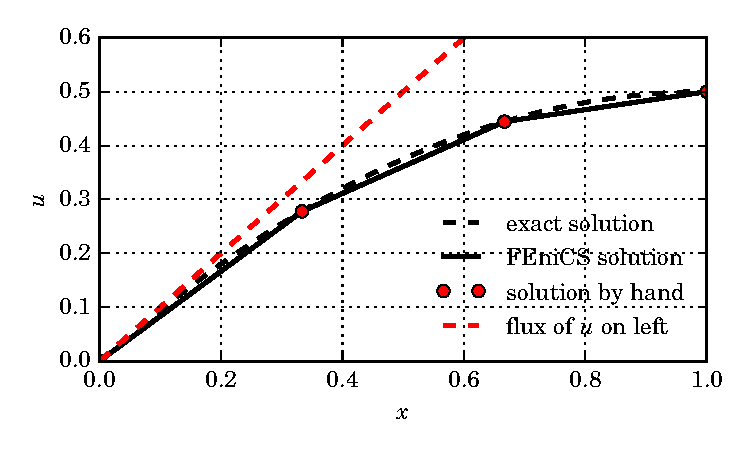
\includegraphics[width=\linewidth]{images/fenics_intro/scratch_example.pdf}
  \caption[Introductory FEM example solution]{Finite element solution computed with FEniCS (solid black), solved exactly (dashed black), and manual finite element (red dots).  The slope $Q_1 = 1$ is shown in dashed red.}
  \label{scratch_ex_image}
\end{figure}

%===============================================================================

\section{FEniCS framework}

The FEniCS ([F]inite [E]lement [ni] [C]omputational [S]oftware) \index{FEniCS} package for python and C++ is a set of packages for easily formulating finite element solutions for differential equations \citep{logg_2012}.  This software includes tools for automatically creating a variety of finite element function spaces, differentiating variational functionals, creating finite element meshes, and much more.  It also includes several linear algebra packages for solving the element equations, including PETSc, uBLAS, Epetra, and MTL4.

For example, the finite element code for introductory problem (\ref{intro_ode} -- \ref{intro_ode_ebc}) is presented in Code Listing \ref{scratch_example_code}.  Notice that only the variational form of the problem is required to find the approximate solution.

\pythonexternal[label=scratch_example_code, caption={FEniCS source code for the introductory problem.}]{scripts/fenics_intro/scratch_example.py}
